\chapter{proposes Framework}

\section{Overview}

The system aims to develop an automated system for agriculture 
that is useful for farmers, agricultural companies and agricultural 
engineers via performing the main agricultural tasks accurately to 
save time and effort by using deep learning to solve the problems 
faced by farmers such as:
\begin{enumerate}
    \item Crop identification
    \item Identification of diseases
    \item Determining the stage of maturity to help determine the quantity 
        of the crop for local use and the quantity of the crop for export.
\end{enumerate}
Early detection of the disease helps farmers to make the right 
decision about treatment and preventive things such as:
\begin{itemize}
    \item Fertilizers.
    \item Herbicides.
    \item Insecticides.
\end{itemize}
To increase the production of the crop. Figure (\ref{fig:plantIdDis}) shows 
the proposed plant identificatoin and diseases detection system using Inception-v3.
\begin{figure}[H]
    \centering
    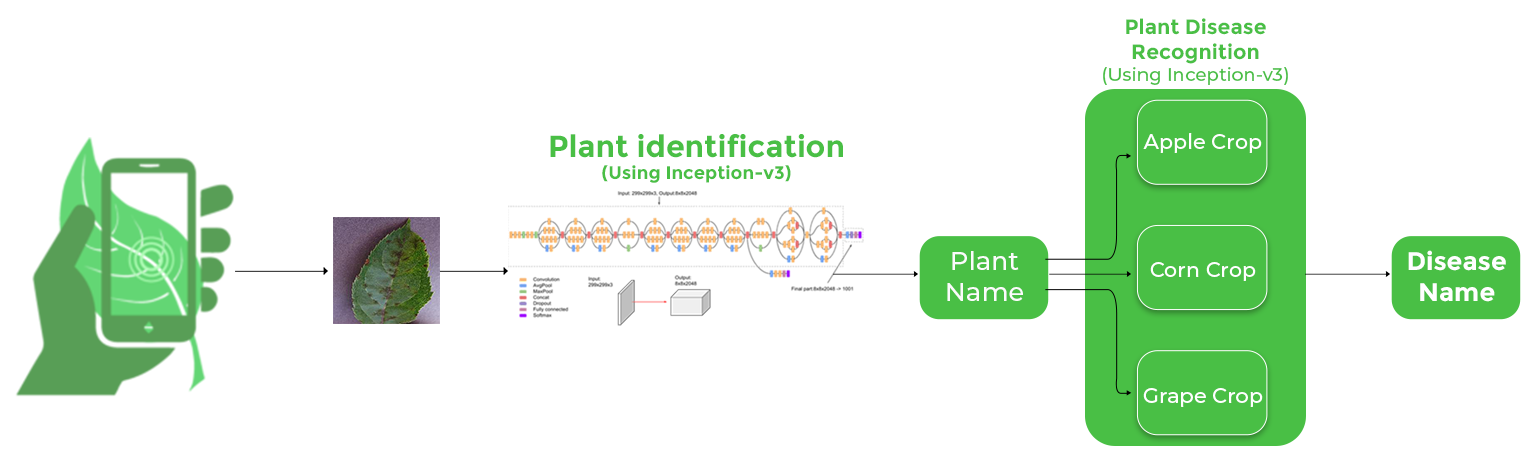
\includegraphics[width=0.9\textwidth]{photos/chapter04/1.png}
    \caption{Plant Identificatoin and Diseases Detection Using Inception-v3.}
    \label{fig:plantIdDis}
\end{figure}

\begin{figure}[H]
    \centering
    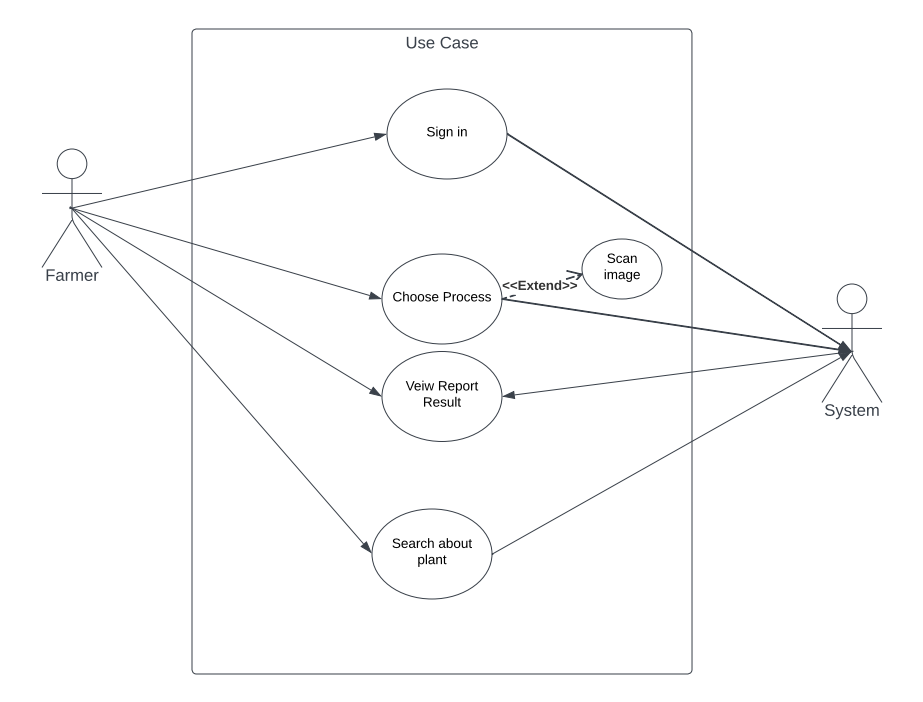
\includegraphics[height=9.5cm]{photos/chapter04/2.png}
    \caption{System Use Case Diagram.}
    \label{fig:systemusecase}
\end{figure}

\section{Sign in Process}

% Figure (\ref{fig:systemusecase}) shows the use case diagram of login process. 
Logon is the procedure used to get access to application. 
Usually a logon requires that the user have (1) a user ID 
and (2) a password. Often, the user ID must conform to a 
limited length. The user ID can be freely known and is visible
when entered at a keyboard or other input device. The password 
must be kept secret (and is not displayed as it is entered). 
Figure (\ref{fig:signupusecase}) shows the use case diagram of sign up and registration process.
\begin{figure}[H]
    \centering
    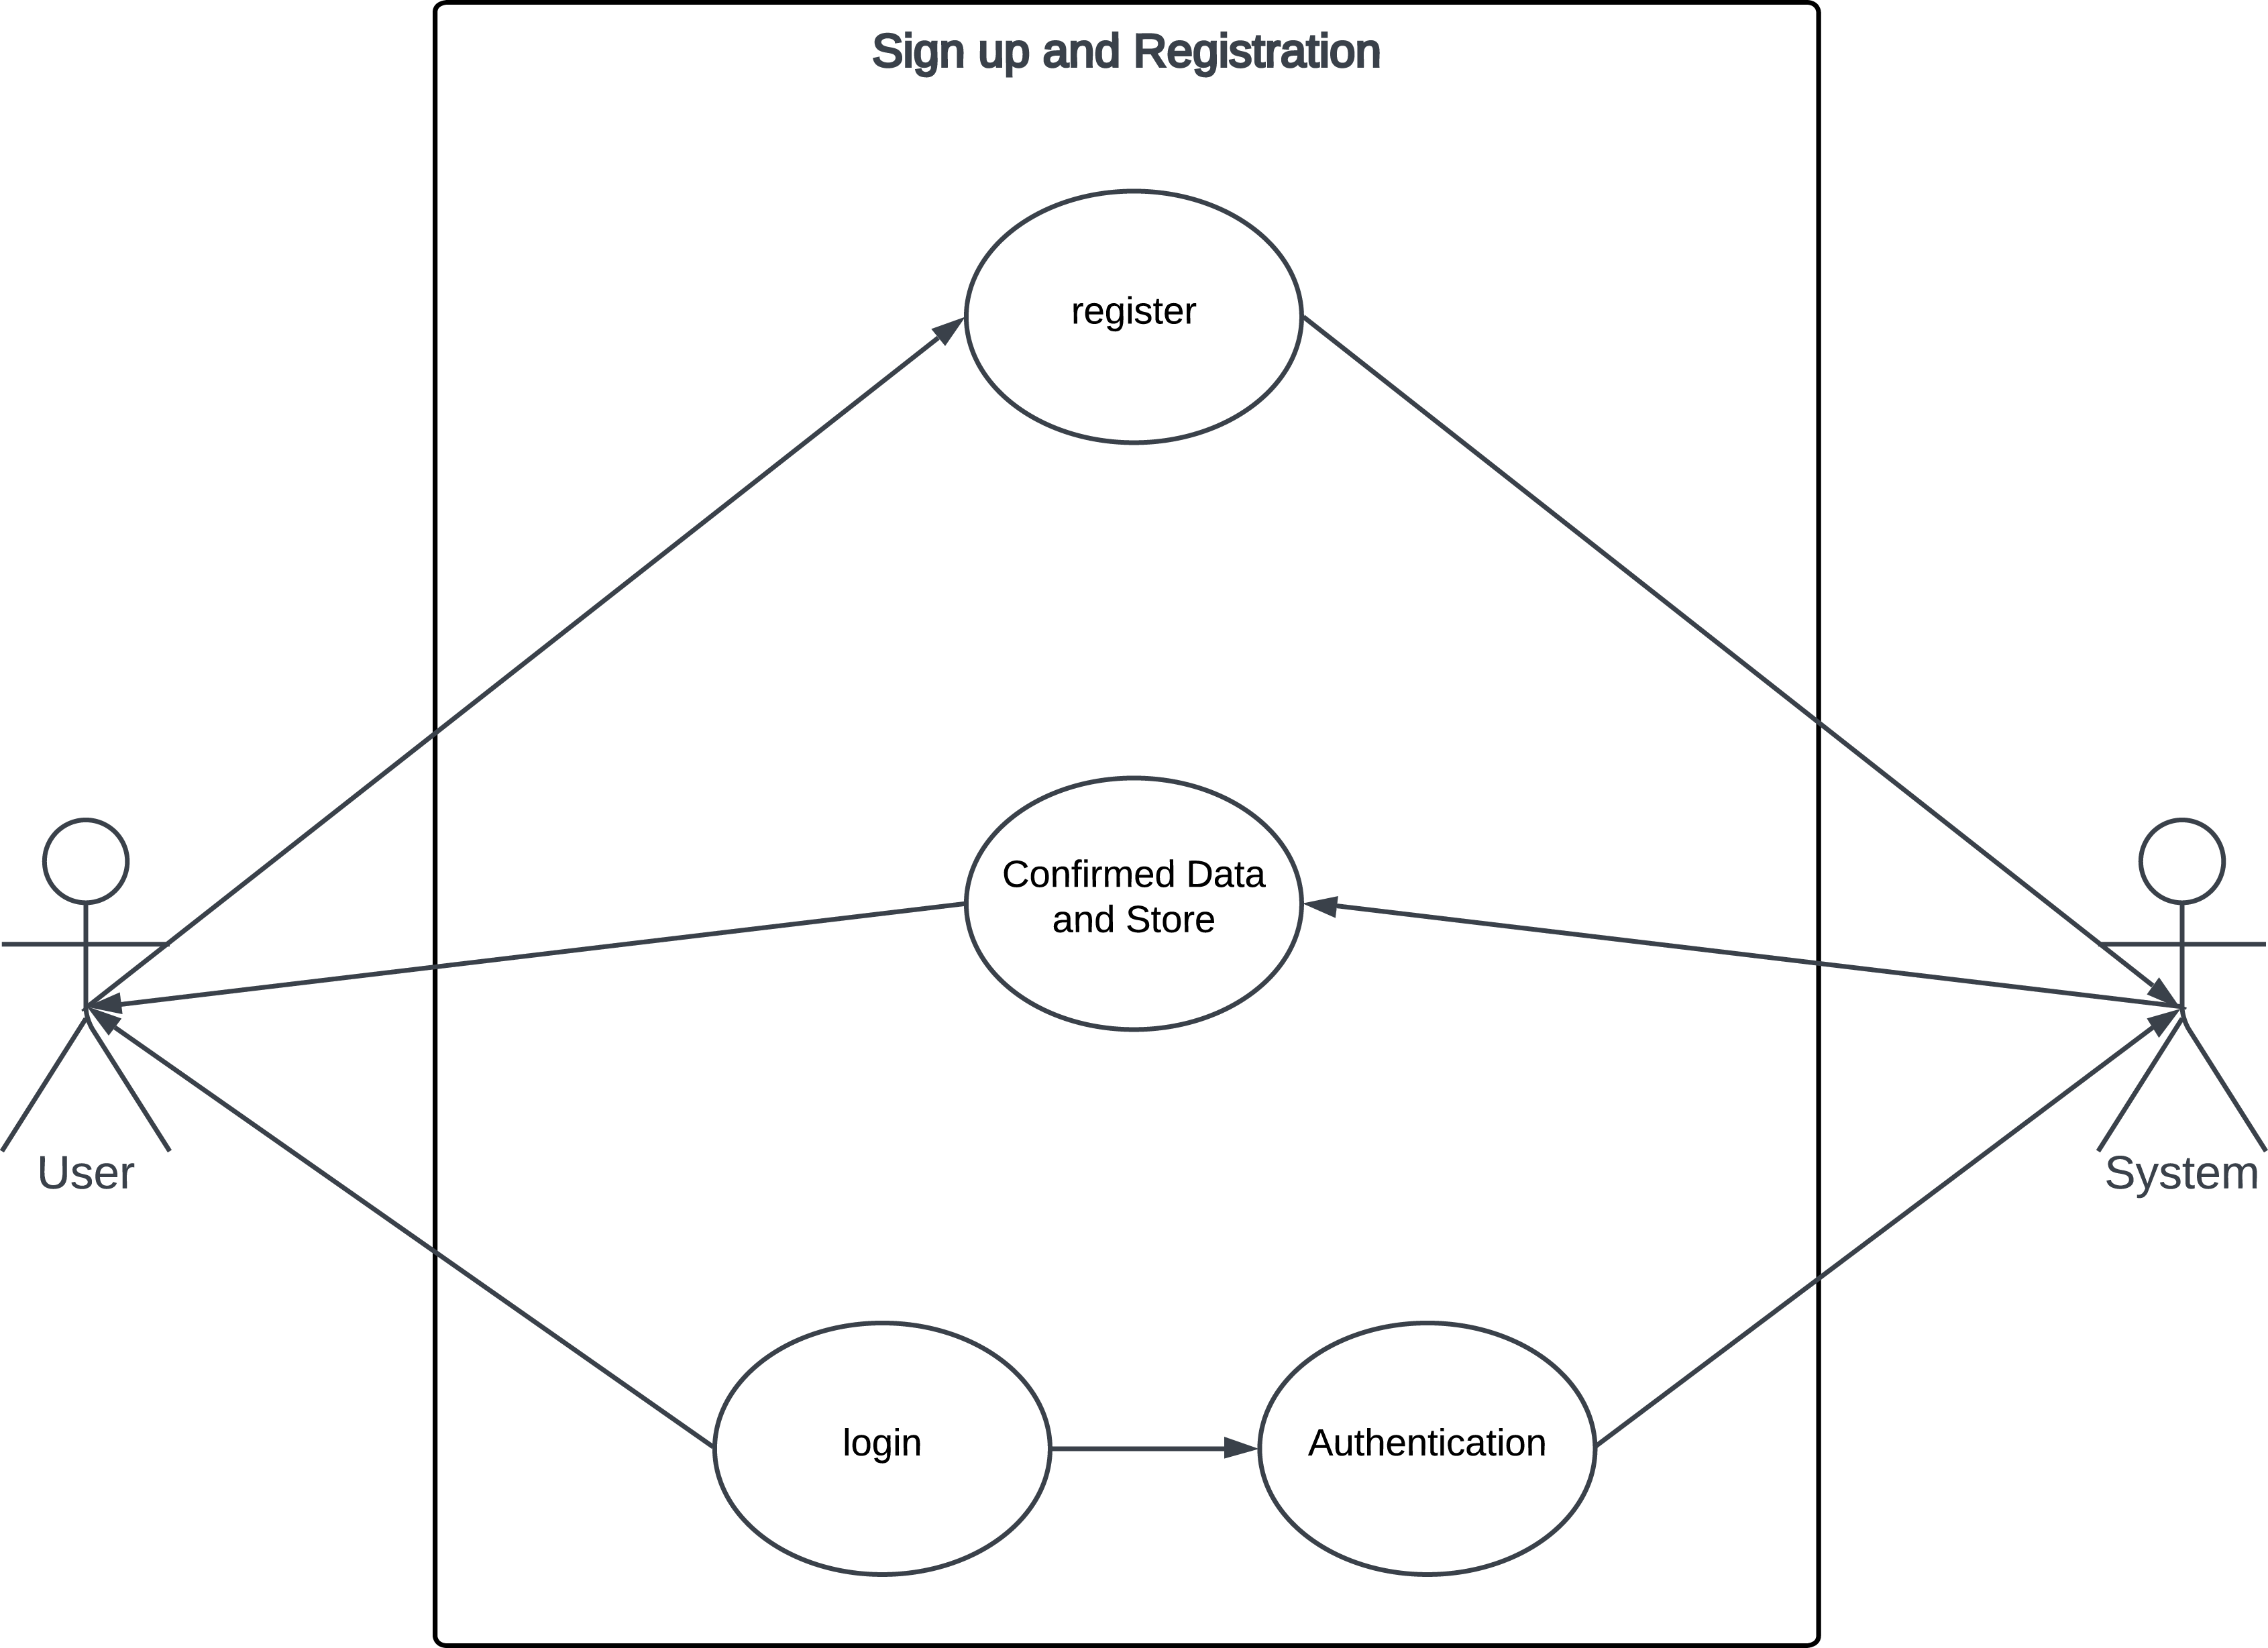
\includegraphics[height=8cm]{photos/chapter04/3.png}
    \caption{Sign Up and Registration Use Case Diagram.}
    \label{fig:signupusecase}
\end{figure}

\noindent Table (\ref{tab:signupscenario}) decribes the "Sign Up" Use Case Scenario.
\begin{table}[H]
    \setlength\arrayrulewidth{0.5pt}
    \renewcommand{\arraystretch}{1.5}%
    \begin{tabularx}{\textwidth}{|>{\columncolor[HTML]{EFEFEF}}l |X|X|}
        \hline
        \textbf{Use case name:} & \multicolumn{2}{l|}{Sign Up} \\ \hline
        \textbf{Actor(s):}      & \multicolumn{2}{l|}{Farmer} \\ \hline
        \textbf{Description:}   
            & \multicolumn{2}{l|}{\makecell[l]{This use case describes sign up steps to our \\ Application.}} \\ \hline
        & \multicolumn{1}{c|}{\cellcolor[HTML]{EFEFEF}\textbf{Actor action}} & \multicolumn{1}{c|}{\cellcolor[HTML]{EFEFEF}\textbf{System Response}} \\ \cline{2-3}
        \multirow{-2}{*}{\textbf{Typical of Events:}} 
                                        & \raggedright Step 1: fill registration Form without skip any field - Then Click ok.
                                        & Step 2: confirm with message in your e-mail. \\ \hline
        \textbf{Alternative:} & \multicolumn{2}{l|}{Step 3: show massage error when massing data.} \\ \hline
        \textbf{Precondition:} & \multicolumn{2}{l|}{No Precondition.} \\ \hline
        \textbf{Post condition:} & \multicolumn{2}{l|}{\makecell[l]{Enter your profile or home page.}} \\ \hline
    \end{tabularx}
    \caption{"Sign Up" Use Case Scenario.}
    \label{tab:signupscenario}
\end{table}

\noindent Table (\ref{tab:loginscenario}) decribes the "Login" Use Case Scenario.
\begin{table}[H]
    \setlength\arrayrulewidth{0.3pt}
    \renewcommand{\arraystretch}{1.3}
    \begin{tabularx}{\textwidth}{|>{\columncolor[HTML]{EFEFEF}}l |X|X|}
        \hline
        \textbf{Use case name:} & \multicolumn{2}{l|}{Log in} \\ \hline
        \textbf{Actor(s):}      & \multicolumn{2}{l|}{Farmer} \\ \hline
        \textbf{Description:}   
            & \multicolumn{2}{l|}{\makecell[l]{This use case describes Login steps \\ Application.}} \\ \hline
        & \multicolumn{1}{c|}{\cellcolor[HTML]{EFEFEF}\textbf{Actor action}} & \multicolumn{1}{c|}{\cellcolor[HTML]{EFEFEF}\textbf{System Response}} \\ \cline{2-3}
        \multirow{-2}{*}{\textbf{Typical of Events:}} 
                                        & \raggedright Step 1: logging to website enter username and password.
                                        & Step 2: check your username and password. \\ \hline
        \textbf{Alternative:} & \multicolumn{2}{l|}{Step 3: check your username and password if it error.} \\ \hline
        \textbf{Precondition:} & \multicolumn{2}{l|}{No Precondition.} \\ \hline
        \textbf{Post condition:} & \multicolumn{2}{l|}{\makecell[l]{Enter your profile or home page.}} \\ \hline
    \end{tabularx}
    \caption{"Login" Use Case Scenario.}
    \label{tab:loginscenario}
\end{table}

\noindent Figure (\ref{fig:loginactive}) shows Login Activity Diagram.
\begin{figure}[H]
    \centering
    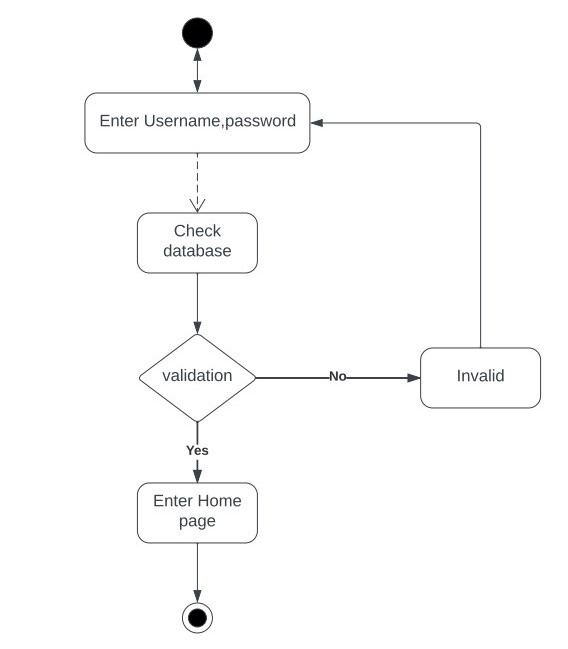
\includegraphics[height=8.5cm]{photos/chapter04/12.jpg}
    \caption{Login Activity Diagram.}
    \label{fig:loginactive}
\end{figure}


\section{Choose Process}
Figure (\ref{fig:chooseprocusecase}) shows Choose Process Use Case Diagram.

\begin{figure}[H]
        \centering
    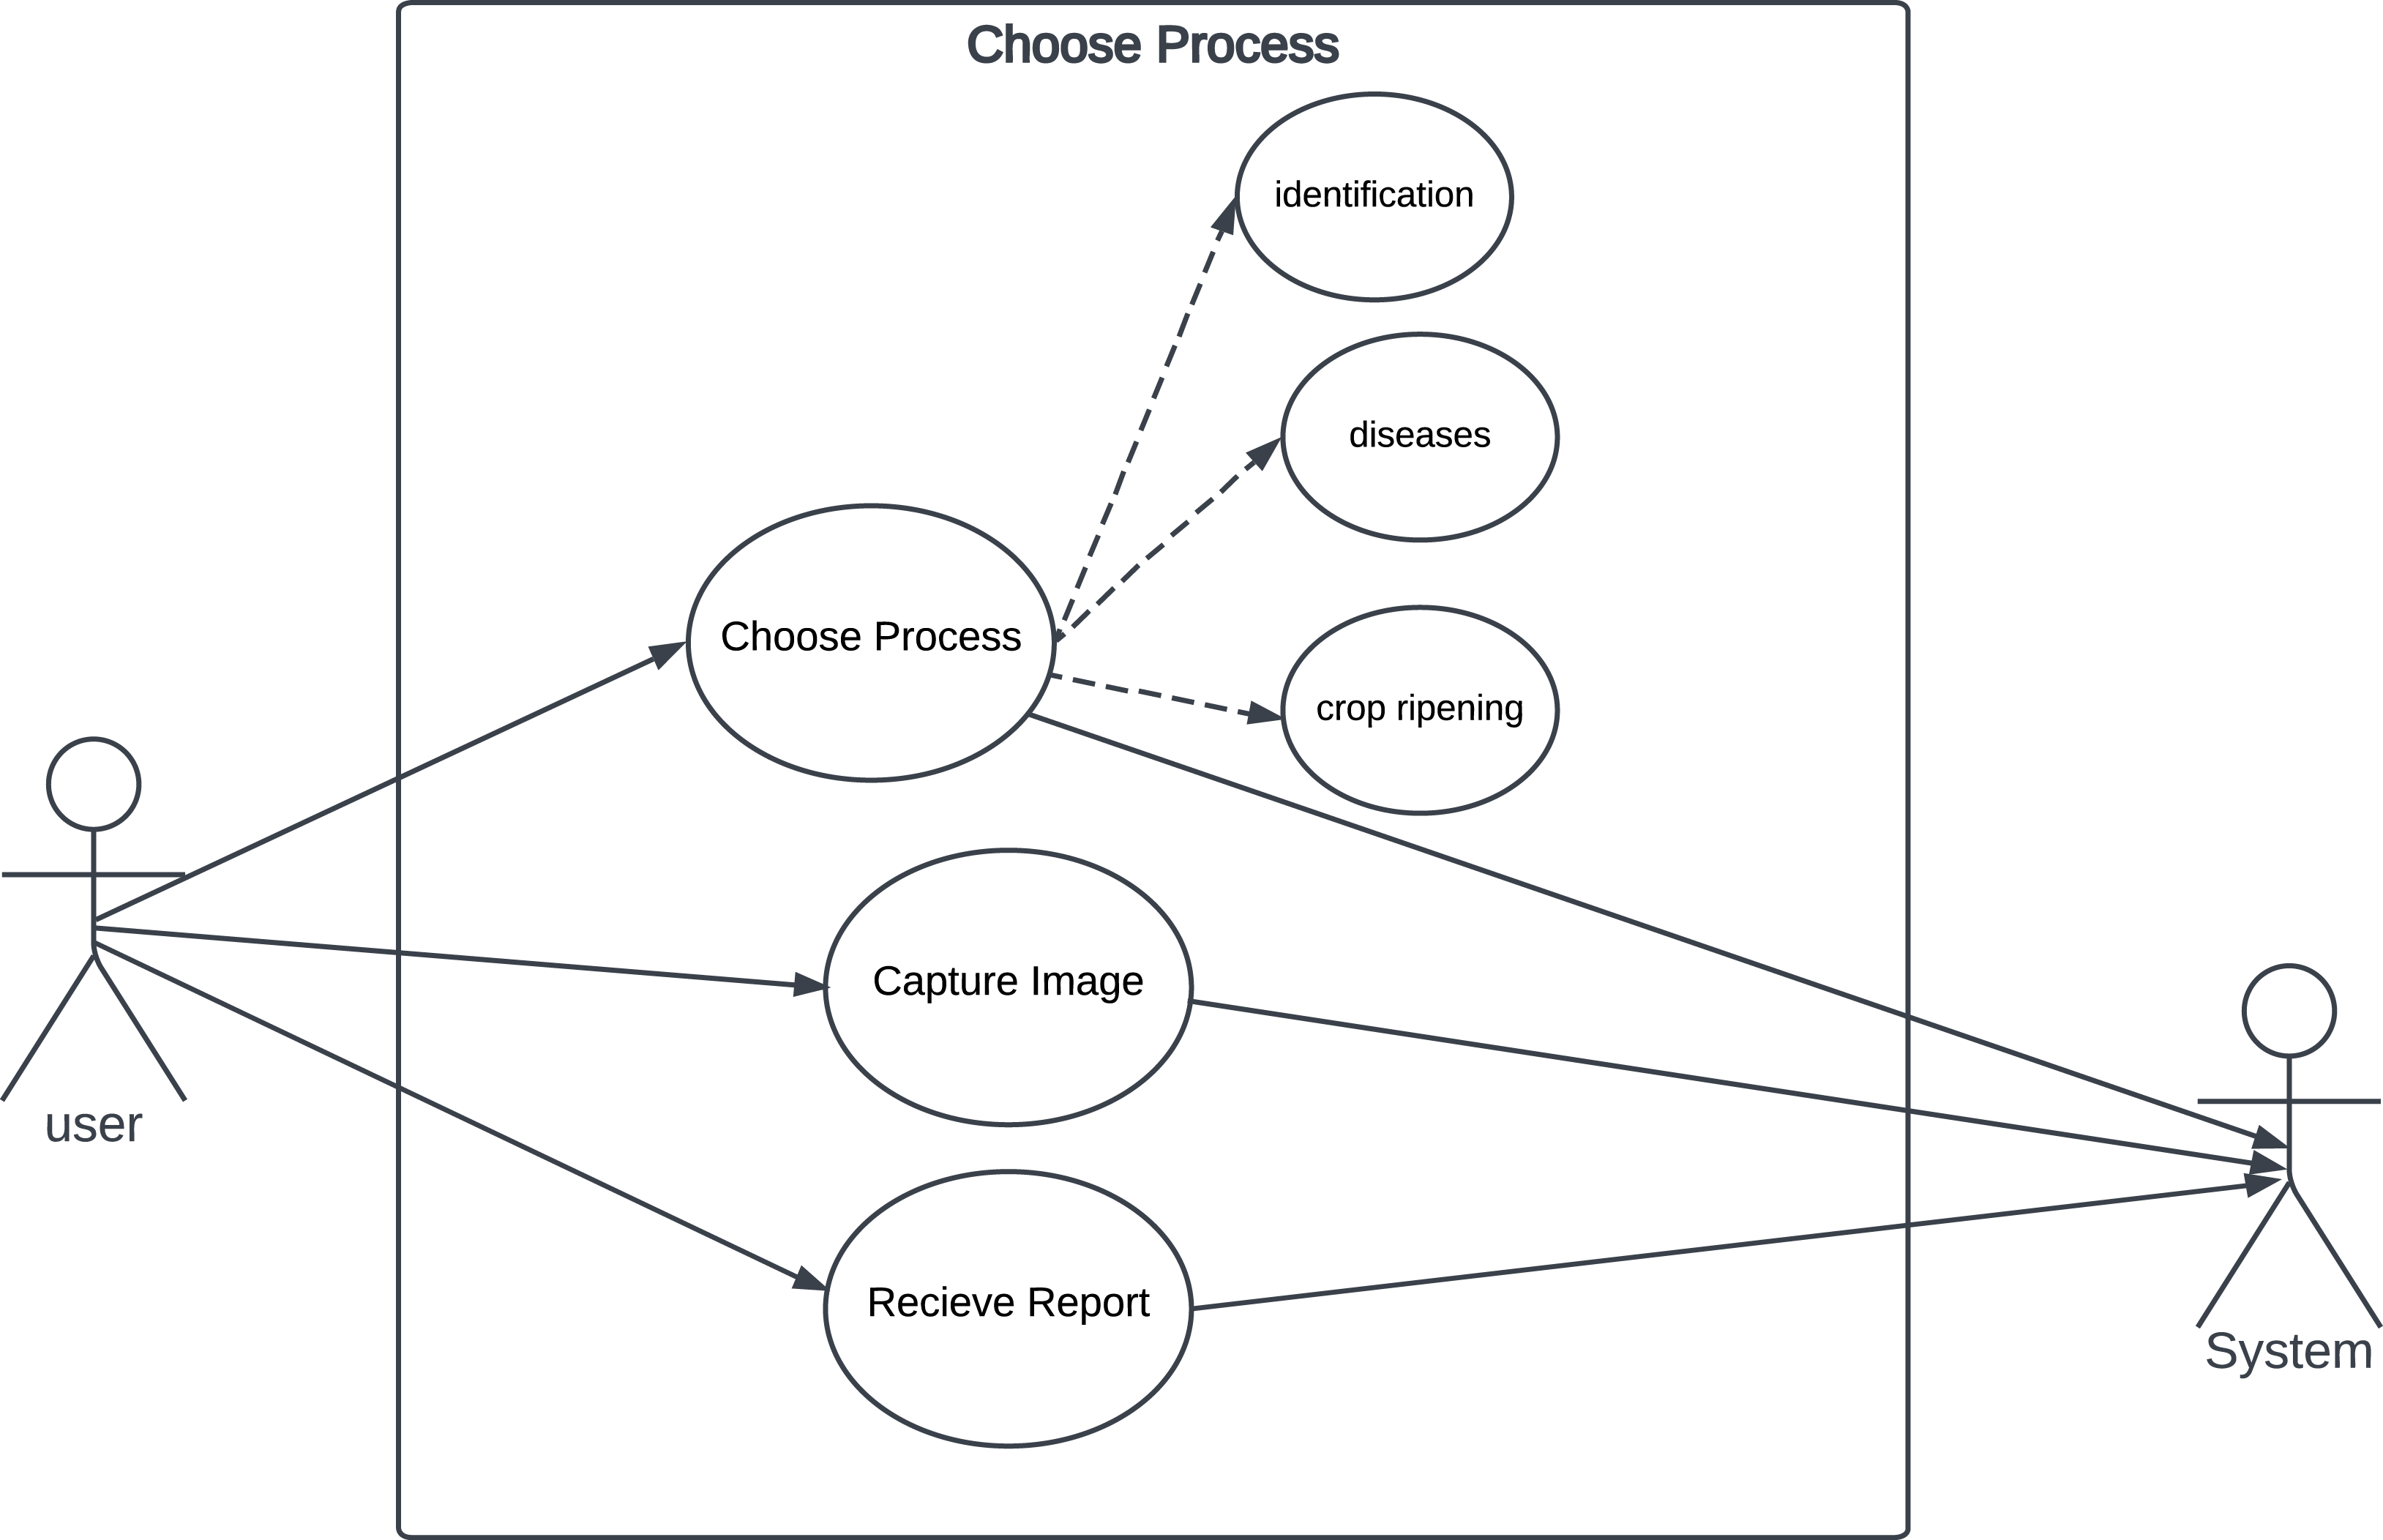
\includegraphics[height=7cm]{photos/chapter04/4.png}
    \caption{Choose Process Use Case Diagram.}
    \label{fig:chooseprocusecase}
\end{figure}

\noindent Table (\ref{tab:chooseprocscenario}) decribes the "Choose Process" Use Case Scenario.
\begin{table}[H]
    \setlength\arrayrulewidth{0.3pt}
    \renewcommand{\arraystretch}{1.2}
    \begin{tabularx}{\textwidth}{|>{\columncolor[HTML]{EFEFEF}}l |X|X|}
        \hline
        \textbf{Use case name:} & \multicolumn{2}{l|}{Choose Process} \\ \hline
        \textbf{Actor(s):}      & \multicolumn{2}{l|}{Farmer} \\ \hline
        \textbf{Description:}   
            & \multicolumn{2}{l|}{\makecell[l]{This use case describes the process that how to choose \\ Process depend What does Farmer want to find out.}} \\ \hline
            & \multicolumn{1}{c|}{\cellcolor[HTML]{EFEFEF}\textbf{Actor action}} 
            & \multicolumn{1}{c|}{\cellcolor[HTML]{EFEFEF}\textbf{System Response}} \\ \cline{2-3}
        \multirow{-2}{*}{\textbf{Typical of Events:}} 
                                        & \raggedright Step 1: this use Application to Choose Process. 
                                        & Step 2: Open Camera to scan image. \\ \hline
        \textbf{Alternative:} & \multicolumn{2}{l|}{Step 3: Choose Image from gallery} \\ \hline
        \textbf{Precondition:} & \multicolumn{2}{l|}{No Precondition.} \\ \hline
        \textbf{Post condition:} & \multicolumn{2}{l|}{\makecell[l]{Response report from disease Page. \\ Record operation in database.}} \\ \hline
    \end{tabularx}
    \caption{"Choose Process" Use Case Scenario.}
    \label{tab:chooseprocscenario}
\end{table}


\subsection{Plants Recognition}

The first process in the system is to determine the type of plant. 
Which is done by taking a picture of your plant, upload it, scan it 
and let the system identify it by performing a preprocessing process
on the image and extracting its features and entering it into the deep
learning model with Inception v3, and view the result in seconds.
Figure (\ref{fig:plantId}) shows The proposed plant identification system.
\begin{figure}[H]
    \centering
    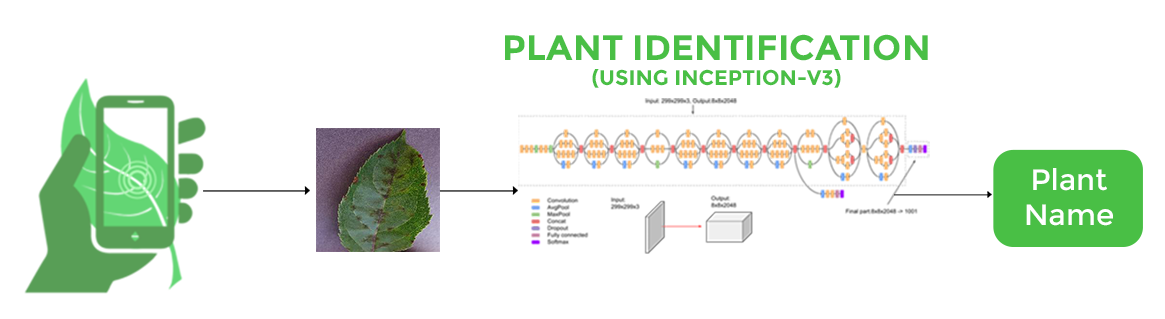
\includegraphics[width=\textwidth]{photos/chapter04/6.png}
    \caption{Plant Identification Model.}
    \label{fig:plantId}
\end{figure}


\subsection{Plants Diseases Recognition}

The second process in the system is plants diseases recognition 
because Plant disease recognition is very critical for agriculture 
due to its importance for increasing crop production. Which is done 
by taking a picture of your plant, upload it, scan it and let the 
system to find out whether this plant has a disease or not, and if 
it has a disease what kind of disease by performing a preprocessing 
process on the image and extracting its features and entering it into 
the deep learning model with Inception v3, and view the result in seconds. 
Figure (\ref{fig:plantDis}) shows The proposed plant diseases recognition system.

\begin{figure}[H]
    \centering
    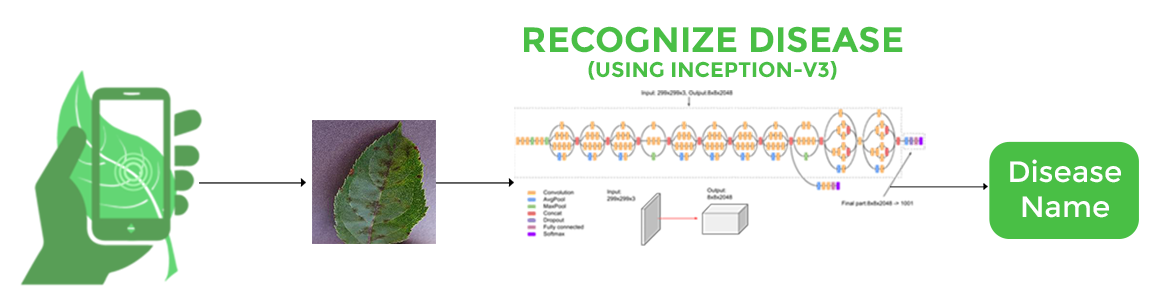
\includegraphics[width=\textwidth]{photos/chapter04/7.png}
    \caption{Plants Diseases Recognition.}
    \label{fig:plantDis}
\end{figure}


\subsection{Ripening Stage}

The third process in the system is recognition ripening stage to
know the time of harvesting the crop for local production and external
export. This is done by taking a picture of your plant, upload it, scan
it and allows the system to know the stage of ripening by performing a
preprocessing process on the image and extracting its features and entering
it into the deep learning model with Inception v3 and view the result in seconds.
Figure (\ref{fig:plantRip}) shows The proposed plant Ripeness rating system.

\begin{figure}[H]
    \centering
    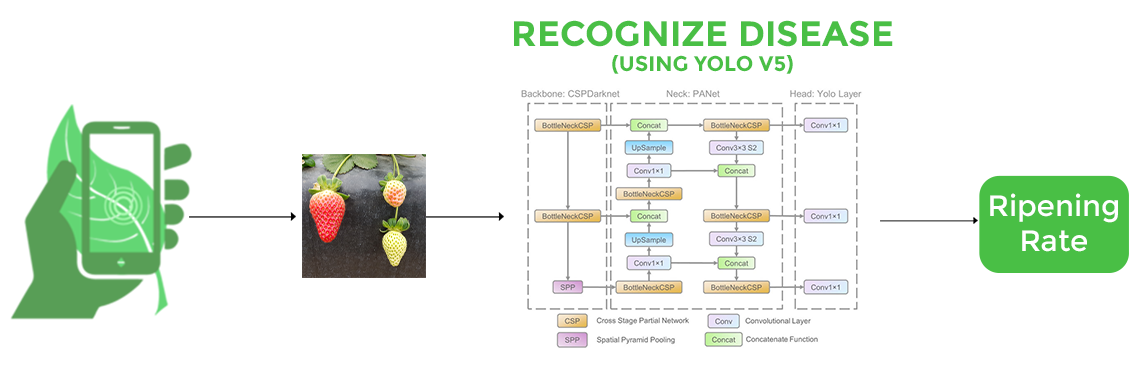
\includegraphics[width=0.8\textwidth]{photos/chapter04/8.png}
    \caption{Plants Ripeness Rating System.}
    \label{fig:plantRip}
\end{figure}


\section{Search Process}
Figure (\ref{fig:searchProcSec}) shows search process sequence diagram.

\begin{figure}[H]
    \centering
    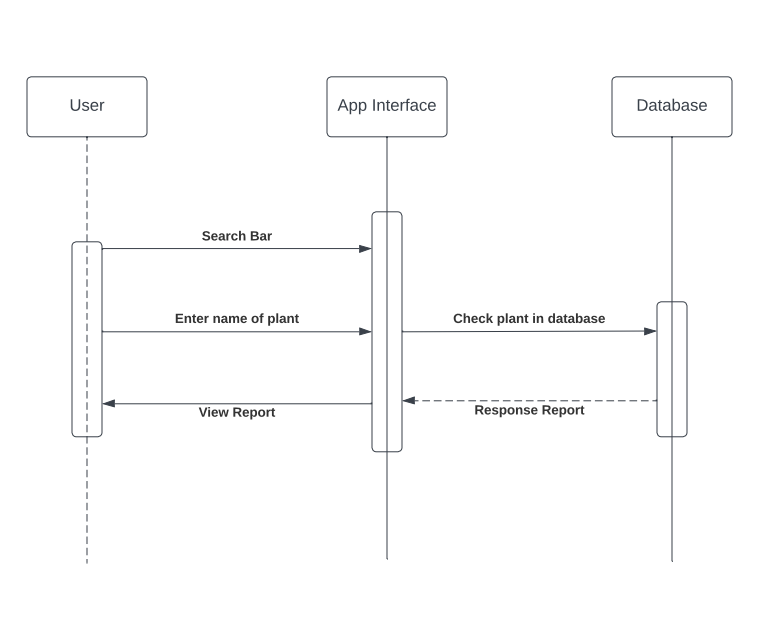
\includegraphics[width=10cm]{photos/chapter04/9.png}
    \caption{Search Process Sequence Diagram.}
    \label{fig:searchProcSec}
\end{figure}

\noindent Figure (\ref{fig:searchProcAtc}) shows search process activity diagram.
\begin{figure}[H]
    \centering
    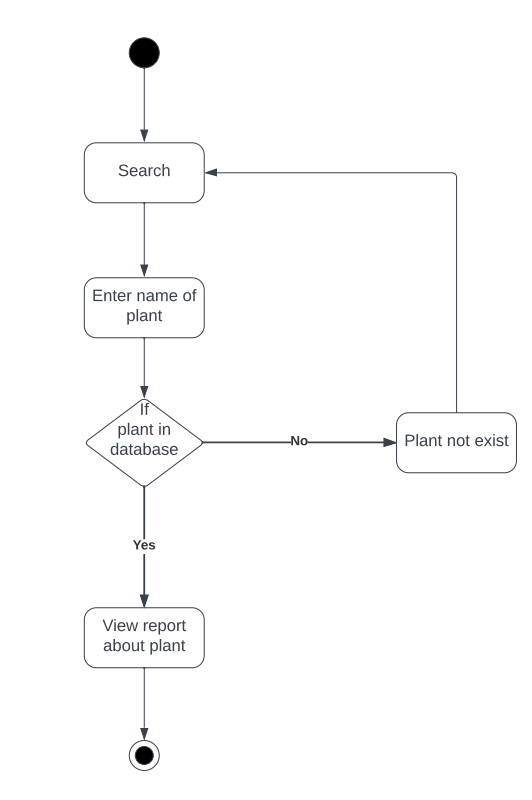
\includegraphics[height=9cm]{photos/chapter04/10.png}
    \caption{Search Process Activity Diagram.}
    \label{fig:searchProcAtc}
\end{figure}

\noindent Figure (\ref{fig:searchProcUse}) shows search process use case diagram.
\begin{figure}[H]
    \centering
    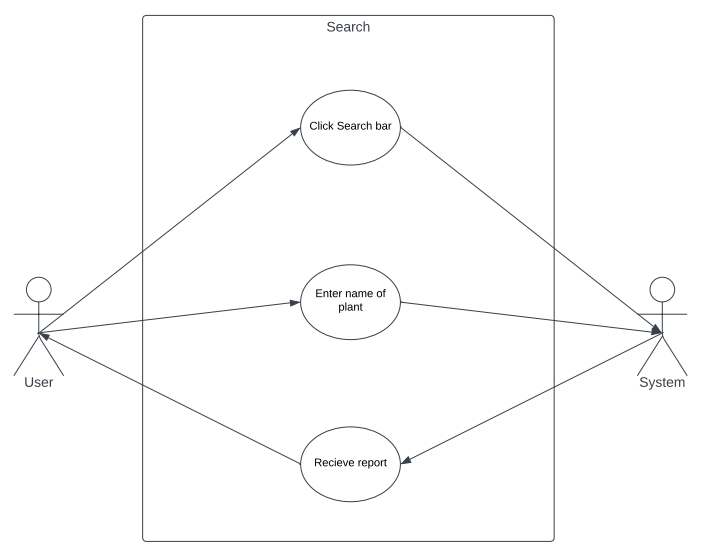
\includegraphics[height=9cm]{photos/chapter04/11.png}
    \caption{Search Process Use Case Diagram.}
    \label{fig:searchProcUse}
\end{figure}

\noindent This system allows the user to search for a plant and know information about
it by entering the name of the plant in the field search bar and the data for
this plant will be displayed.
Table (\ref{tab:searchScenar}) describes "Search" use case scenario.
\begin{table}[H]
    \setlength\arrayrulewidth{0.5pt}
    \renewcommand{\arraystretch}{1.5}
    \begin{tabularx}{\textwidth}{|>{\columncolor[HTML]{EFEFEF}}l |X|X|}
        \hline
        \textbf{Use case name:} & \multicolumn{2}{l|}{Search} \\ \hline
        \textbf{Actor(s):}      & \multicolumn{2}{l|}{Farmer} \\ \hline
        \textbf{Description:}   & \multicolumn{2}{l|}{\makecell[l]{This use case describes the process that how search \\ about specific plant.}} \\ \hline
        & \multicolumn{1}{c|}{\cellcolor[HTML]{EFEFEF}\textbf{Actor action}} & \multicolumn{1}{c|}{\cellcolor[HTML]{EFEFEF}\textbf{System Response}} \\ \cline{2-3}
        \multirow{-2}{*}{\textbf{Typical of Events:}} 
                                        & \raggedright Step 1: this use Application to search about specific plant Enter name of plant. 
                                        & Step 2: check in database if the plant is exist or not. \\ \hline
        \textbf{Alternative:} & \multicolumn{2}{l|}{Step 3: Use identification plant and capture plant.} \\ \hline
        \textbf{Precondition:} & \multicolumn{2}{l|}{No Precondition.} \\ \hline
        \textbf{Post condition:} & \multicolumn{2}{l|}{Response report about plant.} \\ \hline
    \end{tabularx}
    \caption{"Search" Use Case Scenario.}
    \label{tab:searchScenar}
\end{table}
